\documentclass{article}
\usepackage{amsmath}    % For math symbols and formatting
\usepackage{amssymb}    % For symbols like \twoheadrightarrow
\usepackage{geometry}   % To adjust page margins
\usepackage{fancyhdr}   % For header and footer customization
\usepackage{tikz}       % For drawing diagrams

% Page layout
\geometry{a4paper, margin=1in}

% Header and Footer
\pagestyle{fancy}
\fancyhf{}
\lhead{Haskell Notes}
%\rhead{Class Notes}
\cfoot{\thepage}

% Title and Author
\title{\textbf{Haskell Notes}}
\author{Mauro Arcidiacono}
\date{November -- December 2024}

\begin{document}

\maketitle

\section*{Equivalence Relation}

A relation $R \subseteq S \times S$ is an \textbf{equivalence relation} whenever, for $s, t, u \in S$:
\begin{itemize}
    \item $R$ is \textbf{reflexive}, i.e., $(s, s) \in R$;
    \item $R$ is \textbf{symmetric}, i.e., if $(s, t) \in R$, then $(t, s) \in R$;
    \item $R$ is \textbf{transitive}, i.e., if $(s, t) \in R$ and $(t, u) \in R$, then $(s, u) \in R$.
\end{itemize}

This definition applies to various contexts in mathematics and computer science. Equivalence relations are useful in defining partitions of sets and modeling relationships like equality, congruence, or similarity.

\textbf{Define the Renaming} $[y/x]$, \textbf{in the most general way:}
\begin{itemize}
    \item regardless of the free/bound/binding position,
    \item to be applied only if $y$ does not occur in $M$.
\end{itemize}

\[
x[y/x] \equiv y
\]

\[
z[y/x] \equiv z \quad \text{if } x \neq z
\]

\[
(MN)[y/x] \equiv (M[y/x])(N[y/x])
\]

\[
(\lambda x.M)[y/x] \equiv \lambda y.(M[y/x])
\]

\[
(\lambda z.M)[y/x] \equiv \lambda z.(M[y/x]) \quad \text{if } x \neq z
\]
\section*{$\alpha$-Equivalence Relation}

Define when two lambda-terms are \textbf{"the same up to renaming of bound variables"}.

\subsection*{Definition}
\textbf{$\alpha$-equivalence}: The smallest congruence relation on $\lambda$ terms such that for all terms $M$ and all variables $y$ that do not occur in $M$:
\[
\lambda x.M =_\alpha \lambda y.(M[y/x])
\]

\subsection*{Key Properties}
\begin{itemize}
    \item \textbf{"Equivalence"}: must satisfy reflexivity, symmetry, and transitivity.
    \item It must respect the structures of lambda terms and the free/bound occurrences therein:

    \begin{itemize}
        \item If $M = M'$ and $N = N'$, then: $MN = M'N'$
        \item If $M = M'$, then: $\lambda x.M = \lambda x.M'$
        \item If $y \notin M$, then: $\lambda x.M = \lambda y.(M'[y/x])$
    \end{itemize}
\end{itemize}

\section*{$\beta$-Equivalence Relation}

\subsection*{Definition}
$\to_\beta$ is the smallest relation on terms such that:
\begin{itemize}
    \item $(\lambda x.M)N \to_\beta M[N/x]$
    \item if $M \to_\beta M'$, then $MN \to_\beta M'N$
    \item if $N \to_\beta N'$, then $MN \to_\beta MN'$
    \item if $M \to_\beta M'$, then $\lambda x.M \to_\beta \lambda x.M'$
\end{itemize}

\subsection*{$\beta$-Equivalence}
\textbf{$\beta$-equivalence} is the smallest equivalence relation, denoted by $=_\beta$, between pairs of terms, obtained by taking the reflexive, symmetric, and transitive closure of the relation $\to_\beta$.

section*{$\beta$-Equivalence and Normal Forms}

\begin{itemize}
    \item A term that has no redexes is in \textbf{normal form}.
    \item Not all terms have a normal form. For example, the term $\Omega$:
    \[
    (\lambda x.xx)(\lambda x.xx)
    \]
    has a redex, but it $\beta$-reduces to itself, without ever terminating.
    \item Other terms have different computations, all reaching the \textbf{normal form}:
\end{itemize}

\[
(\lambda x.x)((\lambda z.zz)(\lambda y.y)) \to_\beta (\lambda z.zz)(\lambda y.y) \to_\beta (\lambda y.y)(\lambda y.y) \to_\beta \lambda y.y
\]

\[
(\lambda x.x)((\lambda z.zz)(\lambda y.y)) \to_\beta (\lambda x.x)((\lambda y.y)(\lambda y.y)) \to_\beta (\lambda y.y)(\lambda y.y) \to_\beta \lambda y.y
\]

\[
(\lambda x.x)((\lambda z.zz)(\lambda y.y)) \to_\beta (\lambda x.x)((\lambda y.y)(\lambda y.y)) \to_\beta (\lambda x.x)(\lambda y.y) \to_\beta \lambda y.y
\]

\textit{... these are different reduction strategies!}

\section*{Church-Rosser Theorem and Confluence}

Assume that this multi-step reduction exists, $h > 1$, so that $M =_\beta M'$:
\[
M = M_0' \to_\beta M_1' \to_\beta \cdots \to_\beta M_h' = M'
\]

Church-Rosser theorem then asserts that there is a common reduct $N$ for $M$ and $M'$ that can be reached (with $\beta$-reductions):

\begin{figure}[ht]
    \centering
    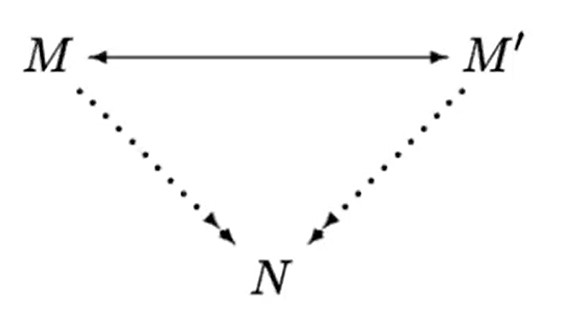
\includegraphics[width=0.2\textwidth]{img/CR_theorem_diagram_0.jpg} % Adjust the width as needed
    \caption{Church Rosser Theorem - Confluence Example 1}
    \label{fig:cr-diagram-1}
\end{figure}

\subsection*{Key Question}
What happens when $M'$ is \emph{a} normal form?
    
    ... and when both $M'$ and $N$ are normal forms?
    
This is about \emph{THE} normal form: if one exists, it is unique.

\begin{figure}[ht]
    \centering
    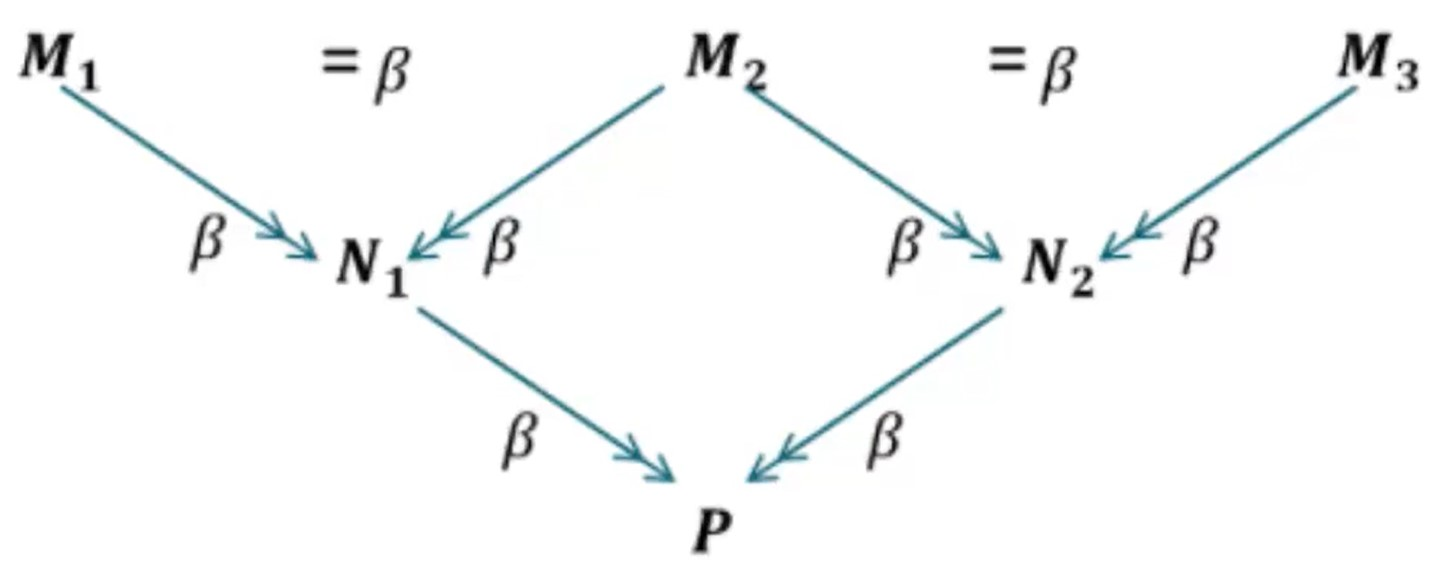
\includegraphics[width=0.5\textwidth]{img/CR_theorem_diagram_1.jpg} % Adjust the width as needed
    \caption{Church Rosser Theorem - Confluence Example 2}
    \label{fig:cr-diagram-2}
\end{figure}

\subsection*{Theorem}
\textbf{Church Rosser Theorem:} For any two $\lambda$-terms $M$ and $N$, $M =_\beta N$ if and only if there is some $\lambda$-term $P$ such that:
\[
M \twoheadrightarrow_\beta^* P \quad \text{and} \quad N \xrightarrow{\beta^*} P
\]

\end{document}
